%----------------------------------------------------------------------------------------
%	PACKAGES & THEMES
%----------------------------------------------------------------------------------------

\pdfminorversion=4
\documentclass[8pt]{beamer}

\usepackage{etex}
\mode<presentation> {

\usetheme{Vilanova}

}



\usepackage[french]{babel}
\usepackage[utf8]{inputenc}
\usepackage{array}
\usepackage{chronology}
\let\CHRONOLOGY\chronology
\let\endCHRONOLOGY\endchronology
\def\chronology{\shorthandoff{;}\CHRONOLOGY}
\def\endchronology{\endCHRONOLOGY\shorthandon{;}}
\usepackage{pstricks}
\usepackage{graphicx}
\usepackage{booktabs}
\usepackage{amsmath,amssymb,amsthm}
\usepackage{xcolor}
\usepackage{tikz}
\usetikzlibrary{arrows}
\usepackage{pifont}

\usepackage{listings,color}

\definecolor{listcomment}{rgb}{0.0,0.5,0.0}
\definecolor{listkeyword}{rgb}{0.0,0.0,0.5}
\definecolor{listnumbers}{gray}{0.65}
\definecolor{listlightgray}{gray}{0.955}
\definecolor{listwhite}{gray}{1.0}


\AtBeginSection[]
{
\addtocounter{framenumber}{-1}
\begin{frame}
\frametitle{Sommaire}
\tableofcontents[currentsection]
\end{frame}}

\title{What's new in Orfeo ToolBox?}
\subtitle{Open source processing of remote sensing images}
\author{Victor Poughon \texttt{\textless victor.poughon@cnes.fr\textgreater}}
\date{2016-06-07}

\pgfdeclareimage[height=96mm,width=130mm]{background}{art/fondsClairSansLogo}
\pgfdeclareimage[height=0.2cm]{cc}{art/CC-licence.png}
\setbeamertemplate{background}{\pgfuseimage{background}}
\pgfdeclareimage[height=0.6cm]{logoIncrust}{art/logoIncrust}
\pgfdeclareimage[height=0.6cm]{logo_cnes}{art/logo_cnes}
\logo{
\begin{tabular}{p{0.22\textwidth}p{0.58\textwidth}p{0.1\textwidth}p{0.1\textwidth}}
\href{http://www.cnes.fr}{\pgfuseimage{logo_cnes}}
& \vspace{-0.03\textwidth} \scriptsize{} % date and event here
& \href{http://creativecommons.org/licenses/by-sa/3.0/}{\pgfuseimage{cc}} & \href{http://www.orfeo-toolbox.org}{\pgfuseimage{logoIncrust}}\\
\end{tabular}
}

\titlegraphic{\vspace*{-5em}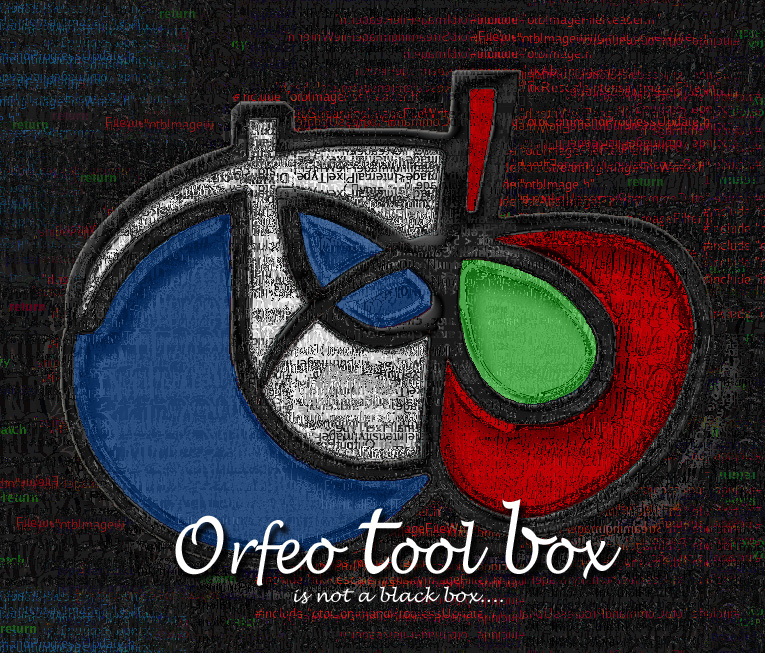
\includegraphics[width=.4\textwidth]{art/LOGOTB_blackbox.png}}

\begin{document}
\begin{frame}
\titlepage
\end{frame}

\section*{Introduction}

\begin{frame}
\frametitle{Si vous ne retenez qu'une planche\ldots}
\begin{block}{L'Orfeo ToolBox est:}
\begin{itemize}
\item Une \textbf{bibliothèque de traitement d'images} pour la télédétection
\item \textbf{Un logiciel libre} diffusé sous licence CeCILL-v2 (équivalent à la GPL)
\item \textbf{Financée et développée par le CNES} (principalement)
\item Écrite en \textbf{C++} sur la base d'\href{www.itk.org}{ITK} (imagerie médicale)
\item Construite sur les épaules de géants (ITK, GDAL, OSSIM, OpenCV\ldots)
\item Conçue pour traiter de \textbf{gros volumes de données} de manière transparente grâce au traitement par morceaux et à la parallélisation
\end{itemize}
\end{block}

\begin{center}
{\huge\textcolor{red}{\href{http://www.orfeo-toolbox.org}{orfeo-toolbox.org}}}
\end{center}

\end{frame}

\begin{frame}
\frametitle{Pourquoi un logiciel libre ?}

\begin{block}{Diffusion maximale}
L'OTB est un logiciel à destination de tous les utilisateurs d'imagerie
spatiale. Sa diffusion large contribue au rayonnement des missions (Pléiades, Sentinels\ldots)
\end{block}

\begin{block}{Qualité et efficacité}
Le domaine fonctionnel de l'OTB est vaste, son développement nécessite du temps
et de l'expertise. L'ouverture des sources favorise:
\begin{itemize}
\item L'appropriation et la validation par la communauté des utilisateurs,
\item Les contributions et les corrections de bugs par les utilisateurs,
\item La dissémination sur de multiples plateformes.
\end{itemize}
\end{block}

\begin{block}{Démarche scientifique}
L'OTB capitalise une partie de la R\&D du CNES en extraction d'information, l'ouverture des sources permet une démarche de \textbf{recherche reproductible}.
\end{block}

\end{frame}

\section{Fonctionnalités et utilisation}

\begin{frame}
\frametitle{Les grandes familles de fonctionnalités dans l'OTB (forcément incomplètes)}
\begin{itemize}
  \item Pré-traitements
  \item Manipulation d'images et de vecteurs
  \item Détection d'éléments saillants et calcul de primitives
  \item Détection de changement
  \item Réduction de la dimension, traitements hyperspectraux
  \item Segmentation
  \item Classification
\end{itemize}
$\Rightarrow$ Proche de l'état de l'art.
\end{frame}

\begin{frame}[plain]
\hspace*{-11mm}
    \includegraphics[keepaspectratio,height=1.1\paperheight]{art/mayotte2012.png}
\end{frame}

\vspace*{-6.5mm}
\begin{frame}[plain]
\hspace*{-11mm}
    \includegraphics[keepaspectratio,height=1.1\paperheight]{art/mayotte2013.png}
\end{frame}

\vspace*{-6.5mm}
\begin{frame}[plain]
\hspace*{-11mm}
    \includegraphics[keepaspectratio,height=1.1\paperheight]{art/mayotte_mad.png}
\end{frame}

\vspace*{-6.5mm}
\begin{frame}[plain]
\hspace*{-11mm}
\includegraphics[keepaspectratio,height=1.1\paperheight]{art/saint_paul_lsd.png}
\end{frame}

\vspace*{-6.5mm}
\begin{frame}[plain]
\hspace*{-11mm}
    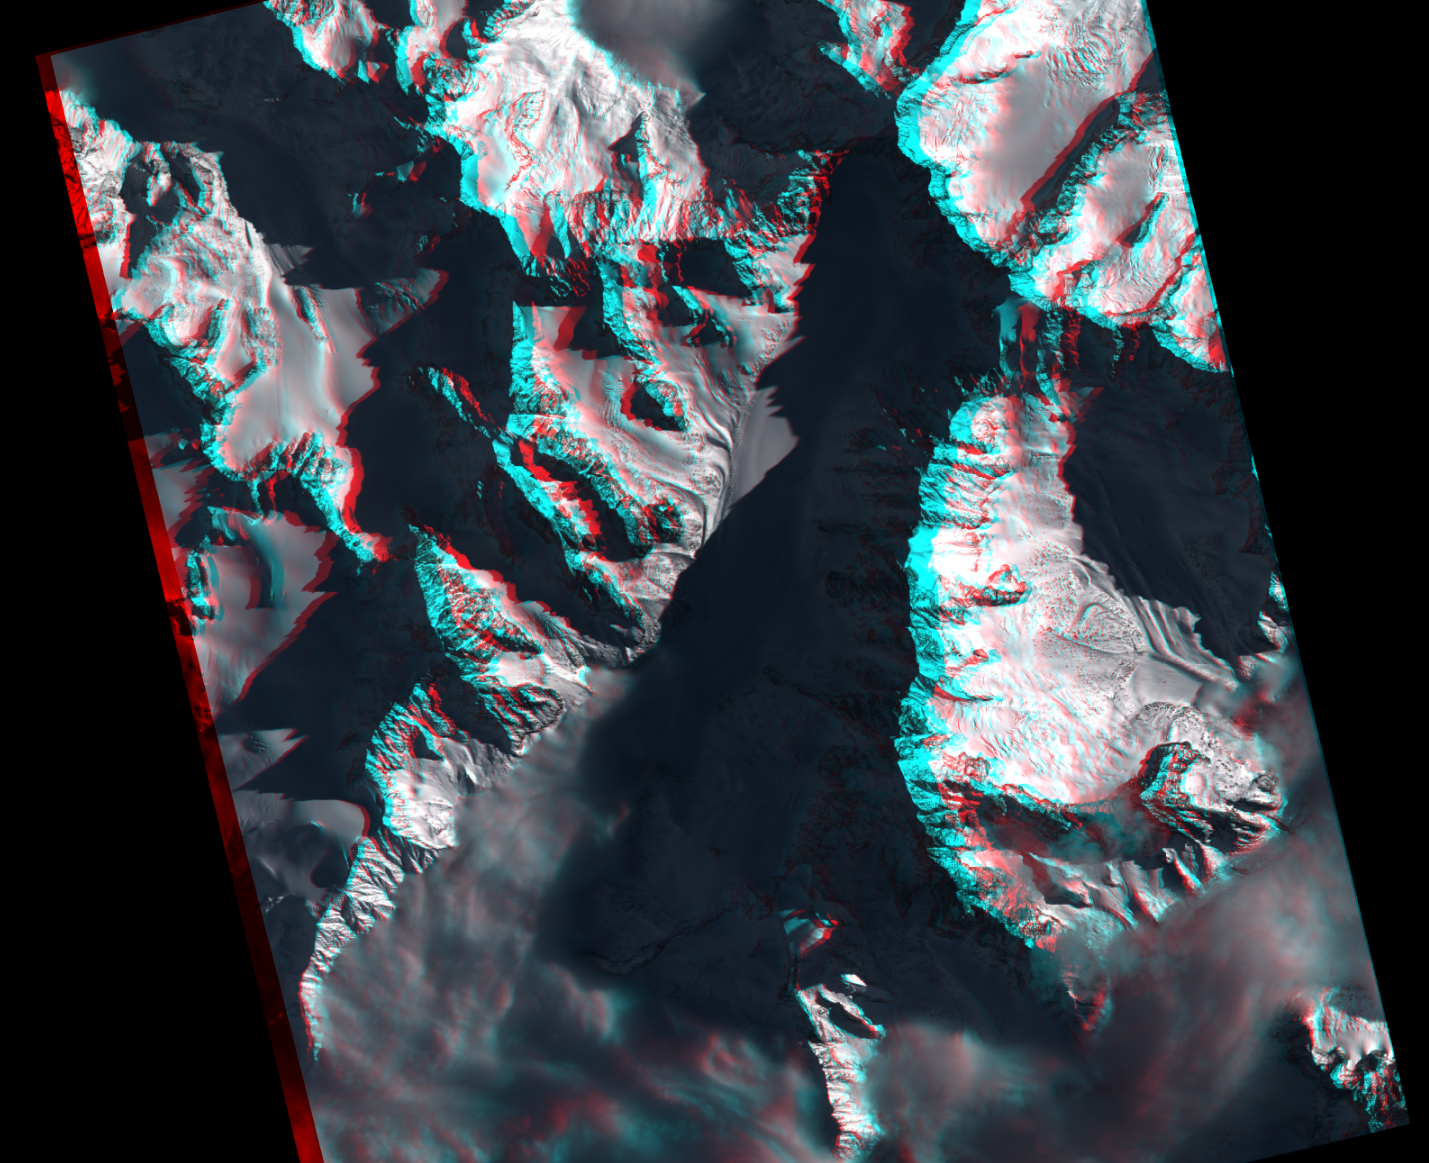
\includegraphics[keepaspectratio,width=1.005\paperwidth,height=1.1\paperheight]{art/argentiere_anaglyphe.png}
\end{frame}

\begin{frame}
\frametitle{Comment utiliser l'Orfeo ToolBox?}
\vspace{-0.5cm}
\begin{center}
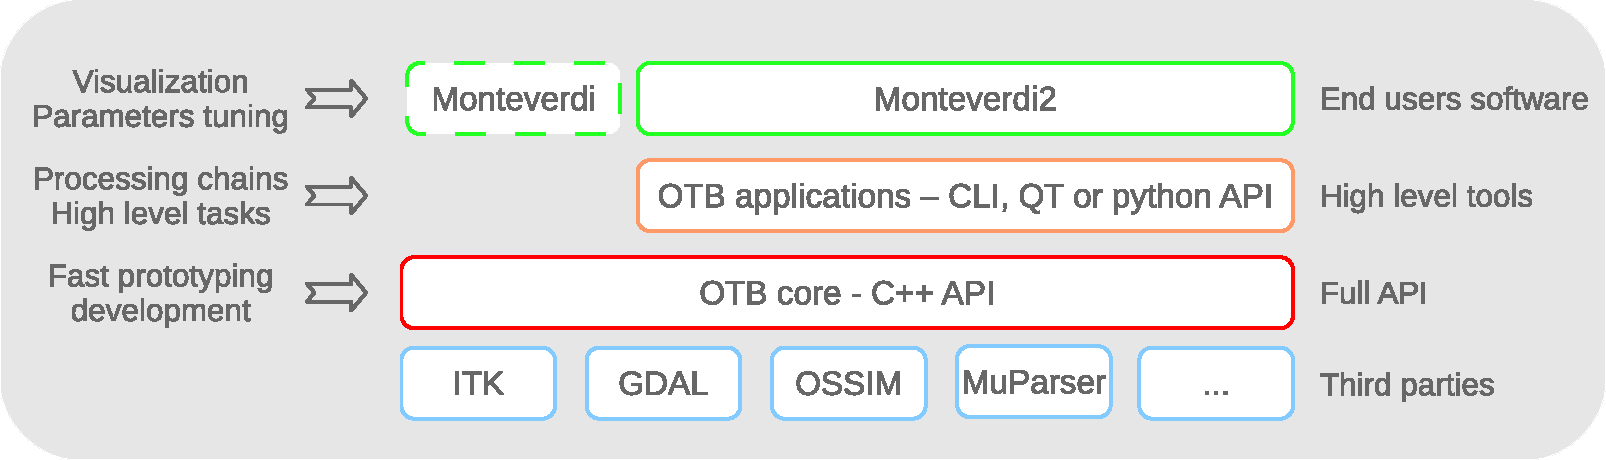
\includegraphics[width=\textwidth]{art/sandwich.pdf}
\end{center}
\vspace{-0.5cm}
\begin{block}{Écrire son propre code}
 Flexible, à partir de la bibliothèque OTB, demande une connaissance en C++
\end{block}
\begin{block}{Utiliser les applications OTB}
 Fonctions de haut niveau (par ex. segmentation), appelable en ligne de commande, via une interface graphique, ou depuis Python. Peut être étendue (création d'applications)
\end{block}
\begin{block}{Utiliser le module Monteverdi (IHM)}
Visualisation, gestion persistante des données, \textcolor{red}{Accès à l'ensemble des applications}
\end{block}
\end{frame}

\begin{frame}
\frametitle{Monteverdi (accès aux applications OTB)}
\begin{minipage}[t][6cm][t]{\textwidth}
\begin{center}
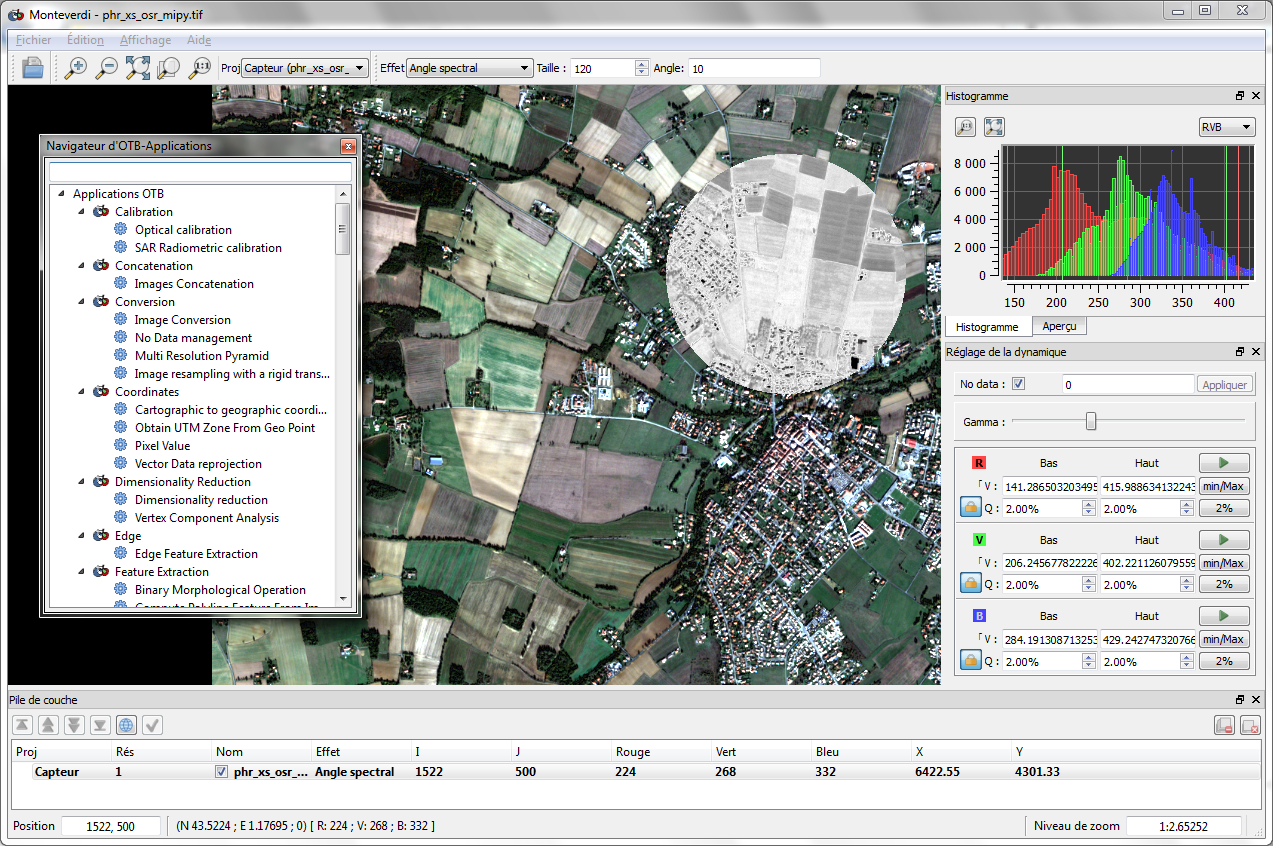
\includegraphics[width=1.0\textwidth]{art/monteverdi.png}
\end{center}
\end{minipage}
\end{frame}

%\vspace*{-3.0mm}
\begin{frame}
  \frametitle{QGIS (accès aux applications OTB)}
\begin{minipage}[t][6cm][t]{\textwidth}
\begin{center}
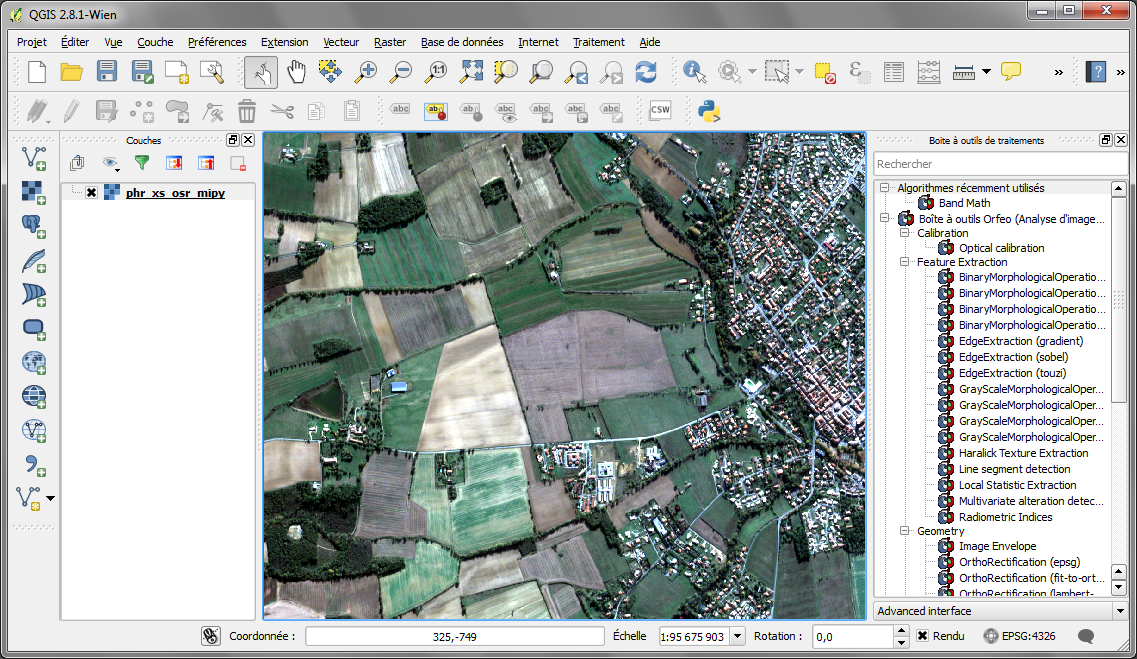
\includegraphics[width=1\textwidth]{art/otb_in_qgis.png}
\end{center}
\end{minipage}
\end{frame}

\section{Quoi de neuf depuis 5.0 ?}

\begin{frame}
\frametitle{5.0 (Mai 2015)}
\begin{block}{Modularité}
\begin{itemize}
\item Une meilleure organisation du code, en modules cohérents (124 modules et
    16 groupes) contenants sources, tests et applications.
\item Gestion des dépendances
\item Contributions externes: \url{https://www.orfeo-toolbox.org/external-projects/}
\end{itemize}
\end{block}

\begin{block}{SuperBuild}
\begin{itemize}
\item Il n'y a plus de logiciels tiers dans l'OTB
\item Le Superbuild, télécharge, configure, compile et installe les dépendances
\item Il existe également un mode \textit{offline} pour compiler l'OTB sans
  accès internet (en avion par exemple).
\end{itemize}
\end{block}
\end{frame}

\begin{frame}
\frametitle{Gouvernance ouverte: Project Steering Committee}
\begin{block}{Genèse du PSC}
  \begin{itemize}
  \item Jusqu'en 2015: l'OTB, un logiciel à sources ouvertes
  \item En mars 2015: l'OTB devient un logiciel libre, le CNES nomme un PSC initial
  \end{itemize}
\end{block}
\begin{block}{Un club de développeurs, pas de décideurs}
  \begin{itemize}
  \item Pilotage haut niveau du projet, roadmaps, communication, planification
  \item Vote les RFCs: Tous les membres ont le même poids dans les votes ($\pm 1$, $\pm 0$)
  \item Les sièges n'expirent pas, sortie par démission ou vote d'expulsion
  \item Le PSC n'est pas une entité légale et n'a pas de moyens propres
  \end{itemize}
\end{block}
\begin{block}{En chiffres}
  \begin{itemize}
  \item 5 membres de 4 entités différentes
  \item 2 release sous l'égide du PSC (5.2, 5.4)
  \item 3 meetings en ligne (logs publics)
  \end{itemize}
\end{block}
\end{frame}

\begin{frame}
\frametitle{5.2 (Décembre 2015)}
\begin{block}{OTB}
\begin{itemize}
\item Nouvelles applications pour le traitement SAR (polarimétrie, radiométrie, speckle)
\item Support des produits Sentinel-1
\item Amélioration accès OTB en Python
\item Compatibilité avec GDAL 2.0 et support des images Sentinel-2
\item \ldots
\end{itemize}
\end{block}

\begin{block}{Monteverdi 3.0}
\begin{itemize}
\item Affichage mosaïque d'images ou série multi-temporelle
\item Outils de visualisation performants (contraste local, gradient\ldots)
\item Accès aux applications OTB
\end{itemize}
\end{block}
\end{frame}

\begin{frame}
\frametitle{5.4 (Mai 2016) Nouveau module d'échantillonnage}
\begin{columns}

\begin{column}{0.6\textwidth}
\begin{block}{Principe}
\begin{itemize}
\item Un nouveau module d'échantillonnage pour l'apprentissage supervisé
\item Différentes méthodes d'échantillonnage: aléatoire, périodique, uniforme.
\end{itemize}
\end{block}
\end{column}

\begin{column}{0.4\textwidth}
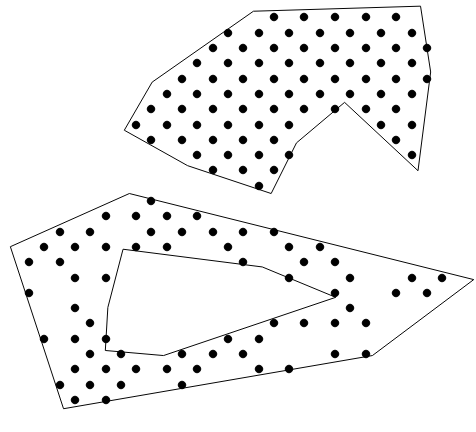
\includegraphics[width=.8\textwidth]{art/sampling.png}
\end{column}
\end{columns}

\begin{center}
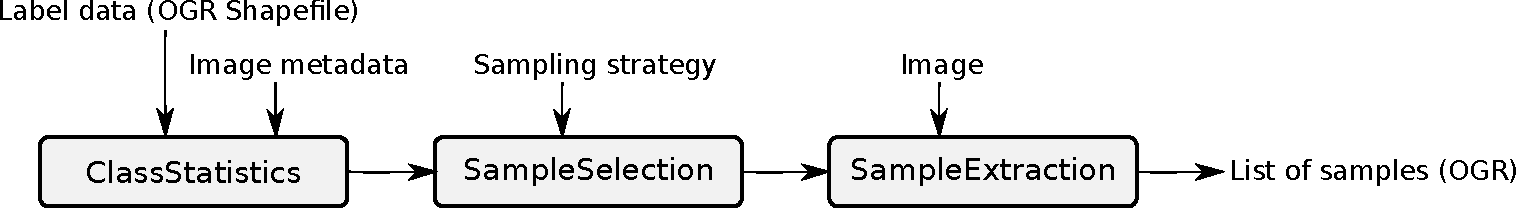
\includegraphics[width=\textwidth]{art/sampling_module.pdf}
\end{center}

\end{frame}

\begin{frame}
\frametitle{5.4 (Mai 2016)}
\begin{block}{OTB}
\begin{itemize}
\item Passage à un cycle de release fixe (3 mois)
\item Intégration du composant de visualisation
\item Compilation externe des modules externes
\item Nouvelles décompositions SAR: Barnes, Huynen, Pauli
\end{itemize}
\end{block}

\begin{block}{Monteverdi 3.2}
\begin{itemize}
\item Capture d'écran
\item Génération d'overviews GDAL
\item Gestion des sous datasets GDAL
\item Ajout au SuperBuild
\end{itemize}
\end{block}
\end{frame}

\section*{Conclusion}

\begin{frame}
\frametitle{Communauté OTB}
\begin{center}
Documentation, blog, wiki, git, bugtracker, dashboard, listes de diffusion:
{\huge\textcolor{red}{\href{http://www.orfeo-toolbox.org}{orfeo-toolbox.org}}}
\end{center}

\begin{block}{Évènements à venir:}
\begin{description}
\item[Journées Utilisateurs OTB] {Du 7 au 9 Juin 2016 à Toulouse}
\item[] {{\footnotesize\url{http://wiki.orfeo-toolbox.org/index.php/OTB\_Users\_meeting\_and\_hackfest\_2016}}}
\item[École d’été OTB et MicMac] {Du 4 au 8 Juillet 2016 à l'ENSG Paris}
\item[] {{\footnotesize\url{http://www.sfpt.fr/2016/04/ecole-dete-logiciels-libres-pour-le-traitement-des-images-satellites/}}}
\end{description}
\end{block}
\begin{center}

\includegraphics[scale=.3]{art/OSGeo_incubation.png}
\end{center}
\end{frame}

\end{document}
